\documentclass[utf8x, 14pt]{G7-32}

% Настройки стиля ГОСТ 7-32
% Для начала определяем, хотим мы или нет, чтобы рисунки и таблицы нумеровались в пределах раздела, или нам нужна сквозная нумерация.
\EqInChapter % формулы будут нумероваться в пределах раздела
\TableInChapter % таблицы будут нумероваться в пределах раздела
\PicInChapter % рисунки будут нумероваться в пределах раздела
\usepackage{slashbox}

\usepackage[table,xcdraw]{xcolor}

% Добавляем гипертекстовое оглавление в PDF
\usepackage[
bookmarks=true, colorlinks=true, unicode=true,
urlcolor=black,linkcolor=black, anchorcolor=black,
citecolor=black, menucolor=black, filecolor=black,
]{hyperref}

% Изменение начертания шрифта --- после чего выглядит таймсоподобно.
\usepackage{cyrtimespatched}

% графика
\usepackage{graphicx}
\graphicspath{ {./img/} }

% отделять первую строку раздела абзацным отступом
\usepackage{indentfirst} 

% Пакет Tikz
\usepackage{tikz}
\usetikzlibrary{arrows,positioning,shadows}

% Произвольная нумерация списков.
\usepackage{enumerate}

% ячейки в несколько строчек
\usepackage{multirow}

% itemize внутри tabular
\usepackage{paralist,array}

% объявляем новую команду для переноса строки внутри ячейки таблицы
\newcommand{\specialcell}[2][c]{%
	\begin{tabular}[#1]{@{}c@{}}#2\end{tabular}}

\usepackage{tikz}
\usepackage{pgfplots}
\usepackage{pdfpages}
\usepackage{caption}
% \captionsetup[table]{position=top}

\usepackage{listings}
\usepackage{xcolor}

\usepackage{setspace}
\usepackage{tabularx}

\makeatletter
\newcommand{\vhrulefill}[1]
{
	\leavevmode\leaders\hrule\@height#1\hfill \kern\z@
}
\makeatother

\makeatletter
\newcommand{\reportheader}[2]
{
	{\centering
		\bf\huge #1 \\ \bf\Large #2\par
	}
}
\makeatother

% \reportstrattr{имяАтрибута}{значение}
\makeatletter
\newcommand{\reportstrattr}[2]
{
	\large\textbf{#1} & \large{#2} \\\cline{2-2} \\
}
\makeatother

\makeatletter
\newcommand{\reportnumattr}[2]
{
	\large\textbf{#1} & \large{#2} \\ \\
}
\makeatother

% \reportstudent{ФИО}{группа}
\makeatletter
\newcommand{\reportstudent}[2]
{
	\large\textbf{Студент} & #2 & & & ~~ & #1 \\
	\cline{2-2} \cline{4-4} \cline{6-6} \vspace{-4mm} \\
	& & & \large\textsuperscript{(подпись, дата)} & &
	\large\textsuperscript{(Фамилия И.О.)} \\
}
\makeatother

% \reporttutor{ФИО}
\makeatletter
\newcommand{\reporttutor}[1]
{
	\large\textbf{Преподаватель} & & & & & #1 \\
	\cline{4-4} \cline{6-6} \vspace{-4mm} \\
	& & & \large\textsuperscript{(подпись, дата)} & &
	\large\textsuperscript{(Фамилия И.О.)} \\
}
\makeatother


% Листинги

\usepackage{listings}
\usepackage{caption}

\usepackage{courier}
\usepackage{wrapfig}

\usepackage{xcolor}
\captionsetup[lstlisting]{singlelinecheck=off, justification=raggedright}


\definecolor{codegreen}{rgb}{0,0.6,0}
\definecolor{codegray}{rgb}{0.5,0.5,0.5}
\definecolor{codepurple}{rgb}{0.58,0,0.82}
\definecolor{backcolour}{rgb}{0.95,0.95,0.92}

\renewcommand{\ttdefault}{cmtt}

% Значения по умолчанию
\lstset{
	% подсветка синтаксиса
	backgroundcolor=\color{white},   
	commentstyle=\color{codegreen},
	keywordstyle=\color{blue},
	numberstyle=\tiny\color{codegray},
	stringstyle=\color{codepurple},
	basicstyle= \footnotesize\ttfamily\bfseries,
	basewidth={.5em,0.5em},
	breakatwhitespace=true,% разрыв строк только на whitespacce
	breaklines=true,       % переносить длинные строки
	% captionpos=b,          % подписи снизу -- вроде не надо
	inputencoding=utf8, %koi8-r,
	numbers=left,          % нумерация слева
	numberstyle=\footnotesize,
	showspaces=false,      % показывать пробелы подчеркиваниями
	showstringspaces=false,
	showtabs=false,        % и табы тоже
	stepnumber=1,
	tabsize=4,              % кому нужны табы по 8 символов?
	frame=single,
	escapeinside={(*}{*)}, %выделение
  literate={а}{{\selectfont\char224}}1
  {б}{{\selectfont\char225}}1
  {в}{{\selectfont\char226}}1
  {г}{{\selectfont\char227}}1
  {д}{{\selectfont\char228}}1
  {е}{{\selectfont\char229}}1
  {ё}{{\"e}}1
  {ж}{{\selectfont\char230}}1
  {з}{{\selectfont\char231}}1
  {и}{{\selectfont\char232}}1
  {й}{{\selectfont\char233}}1
  {к}{{\selectfont\char234}}1
  {л}{{\selectfont\char235}}1
  {м}{{\selectfont\char236}}1
  {н}{{\selectfont\char237}}1
  {о}{{\selectfont\char238}}1
  {п}{{\selectfont\char239}}1
  {р}{{\selectfont\char240}}1
  {с}{{\selectfont\char241}}1
  {т}{{\selectfont\char242}}1
  {у}{{\selectfont\char243}}1
  {ф}{{\selectfont\char244}}1
  {х}{{\selectfont\char245}}1
  {ц}{{\selectfont\char246}}1
  {ч}{{\selectfont\char247}}1
  {ш}{{\selectfont\char248}}1
  {щ}{{\selectfont\char249}}1
  {ъ}{{\selectfont\char250}}1
  {ы}{{\selectfont\char251}}1
  {ь}{{\selectfont\char252}}1
  {э}{{\selectfont\char253}}1
  {ю}{{\selectfont\char254}}1
  {я}{{\selectfont\char255}}1
  {А}{{\selectfont\char192}}1
  {Б}{{\selectfont\char193}}1
  {В}{{\selectfont\char194}}1
  {Г}{{\selectfont\char195}}1
  {Д}{{\selectfont\char196}}1
  {Е}{{\selectfont\char197}}1
  {Ё}{{\"E}}1
  {Ж}{{\selectfont\char198}}1
  {З}{{\selectfont\char199}}1
  {И}{{\selectfont\char200}}1
  {Й}{{\selectfont\char201}}1
  {К}{{\selectfont\char202}}1
  {Л}{{\selectfont\char203}}1
  {М}{{\selectfont\char204}}1
  {Н}{{\selectfont\char205}}1
  {О}{{\selectfont\char206}}1
  {П}{{\selectfont\char207}}1
  {Р}{{\selectfont\char208}}1
  {С}{{\selectfont\char209}}1
  {Т}{{\selectfont\char210}}1
  {У}{{\selectfont\char211}}1
  {Ф}{{\selectfont\char212}}1
  {Х}{{\selectfont\char213}}1
  {Ц}{{\selectfont\char214}}1
  {Ч}{{\selectfont\char215}}1
  {Ш}{{\selectfont\char216}}1
  {Щ}{{\selectfont\char217}}1
  {Ъ}{{\selectfont\char218}}1
  {Ы}{{\selectfont\char219}}1
  {Ь}{{\selectfont\char220}}1
  {Э}{{\selectfont\char221}}1
  {Ю}{{\selectfont\char222}}1
  {Я}{{\selectfont\char223}}1
}

\lstloadlanguages{
  C++
}

% Стиль для псевдокода: строчки обычно короткие, поэтому размер шрифта побольше
\lstdefinestyle{pseudocode}{
  basicstyle=\small,
  keywordstyle=\color{black}\bfseries\underbar,
  language=Pseudocode,
  numberstyle=\footnotesize,
  commentstyle=\footnotesize\it
}

% Стиль для обычного кода: маленький шрифт
\lstdefinestyle{realcode}{
  basicstyle=\scriptsize,
  numberstyle=\footnotesize
}

% Стиль для коротких кусков обычного кода: средний шрифт
\lstdefinestyle{simplecode}{
  basicstyle=\footnotesize,
  numberstyle=\footnotesize
}

% Стиль для BNF
\lstdefinestyle{grammar}{
  basicstyle=\footnotesize,
  numberstyle=\footnotesize,
  stringstyle=\bfseries\ttfamily,
  language=BNF
}

% Определим свой язык для написания псевдокодов на основе Python
\lstdefinelanguage[]{Pseudocode}[]{Python}{
  morekeywords={each,empty,wait,do},% ключевые слова добавлять сюда
  morecomment=[s]{\{}{\}},% комменты {а-ля Pascal} смотрятся нагляднее
  literate=% а сюда добавлять операторы, которые хотите отображать как мат. символы
    {->}{\ensuremath{$\rightarrow$}~}2%
    {<-}{\ensuremath{$\leftarrow$}~}2%
    {:=}{\ensuremath{$\leftarrow$}~}2%
    {<--}{\ensuremath{$\Longleftarrow$}~}2%
}[keywords,comments]

% Свой язык для задания грамматик в BNF
\lstdefinelanguage[]{BNF}[]{}{
  morekeywords={},
  morecomment=[s]{@}{@},
  morestring=[b]",%
  literate=%
    {->}{\ensuremath{$\rightarrow$}~}2%
    {*}{\ensuremath{$^*$}~}2%
    {+}{\ensuremath{$^+$}~}2%
    {|}{\ensuremath{$|$}~}2%
}[keywords,comments,strings]

% Подписи к листингам на русском языке.
\renewcommand\lstlistingname{\cyr\CYRL\cyri\cyrs\cyrt\cyri\cyrn\cyrg}
\renewcommand\lstlistlistingname{\cyr\CYRL\cyri\cyrs\cyrt\cyri\cyrn\cyrg\cyri}

\lstdefinestyle{asm}{
	language={[x86masm]Assembler},
	backgroundcolor=\color{white},
	basicstyle=\footnotesize\ttfamily,
	keywordstyle=\color{blue},
	stringstyle=\color{red},
	commentstyle=\color{gray},
	numbers=left,
	numberstyle=\tiny,
	stepnumber=1,
	numbersep=5pt,
	frame=single,
	tabsize=4,
	captionpos=b,
	breaklines=true
}

\lstdefinestyle{cpp}{
	language={C++},
	backgroundcolor=\color{white},
	basicstyle=\footnotesize\ttfamily,
	keywordstyle=\color{blue},
	stringstyle=\color{red},
	commentstyle=\color{gray},
	numbers=left,
	numberstyle=\tiny,
	stepnumber=1,
	numbersep=5pt,
	frame=single,
	tabsize=4,
	captionpos=b,
	breaklines=true
}


\begin{document}

\frontmatter % выключает нумерацию ВСЕГО; здесь начинаются ненумерованные главы: реферат, введение, глоссарий, сокращения и прочее.

\begin{table}[ht]
	\centering
	\begin{tabular}{|c|p{400pt}|} 
	\hline
		\begin{tabular}[c]{@{}c@{}} 
\includegraphics[scale=0.37]{EmblemBMSTU} \\\end{tabular} &
		\footnotesize\begin{tabular}[c]{@{}c@{}}\textbf{Министерство~науки~и~высшего~образования~Российской~Федерации}\\\textbf{Федеральное~государственное~бюджетное~образовательное~учреждение}\\\textbf{~высшего~образования}\\\textbf{«Московский~государственный~технический~университет}\\\textbf{имени~Н.Э.~Баумана}\\\textbf{(национальный~исследовательский~университет)»}\\\textbf{(МГТУ~им.~Н.Э.~Баумана)}\\\end{tabular}  \\
	\hline
	\end{tabular}
\end{table}
\noindent\rule{\textwidth}{4pt}
\noindent\rule[14pt]{\textwidth}{1pt}
\vspace{-10mm}

\begin{table}[ht]
	\centering
	\begin{tabularx}{\textwidth} {l >{\raggedright\arraybackslash}X }
		\small{ФАКУЛЬТЕТ} & <<Информатика и системы управления>> \\ \cline{2-2} \vspace{-4mm} \\
		\small{КАФЕДРА} & <<Программное обеспечение ЭВМ и информационные технологии>> \\ \cline{2-2}
	\end{tabularx}
\end{table}

\vspace{25mm}
\reportheader{Отчёт}{по лабораторной работе №14}
\vspace{0.5cm}

\begin{table}[h]
	\centering
	\begin{tabularx}{\textwidth} {l >{\raggedright\arraybackslash}X }
		\reportstrattr{Название}{<<Использование правил в программе на Prolog>>}
		\reportstrattr{Дисциплина}{<<Функциональное и логическое программирование>>}
	\end{tabularx}

	\vspace{4cm}

	\begin{tabularx}{\textwidth} {l c >{\centering\arraybackslash}X c c c }		
		\reportstudent{Клименко А.К.}{ИУ7-65Б}
		\reporttutor{Толпинская Н.Б.}
	\end{tabularx}
\end{table}

\begin{center}
	\vfill
	\large \textit {Москва, \the\year}
\end{center}

\thispagestyle {empty}
\pagebreak

\tableofcontents
\pagebreak

{\large\section*{Введение}}

\textbf{Цель работы} -- изучить структуру, особенности и принципы оформления программы, и способ выполнения программы на Prolog.

Для достижения поставленной цели необходимо решить следующие задачи:

\begin{itemize}[$\bullet$]
	\item приобрести навыки декларативного описания предметной области с использованием фактов, правил и некоторых специальных разделов программы.
	\item Изучить порядок использования фактов и правил в программе на Prolog, принципы и особенности сопоставления и отождествления термов, на основе механизма унификации.
\end{itemize}


\mainmatter % это включает нумерацию глав и секций в документе ниже

{\large\section*{Теоритические вопросы}}

\begin{enumerate}
	\item \textit{Какое первое состояние резольвенты?}
	
	\qquad \textbf{Ответ}: первое состояние резольвенты представляет собой вопрос.

	\item \textit{В каком случае система запускает алгоритм унификации? (Как эту необходимость на формальном уровне распознает система?)}

	\qquad \textbf{Ответ}: алгоритм унификации запускается системой в случае необходимости проверить, подходит ли текущее правило в базе знаний для доказательства текущей цели.

	\item \textit{Каковы назначение и результат использования алгоритма унификации?}
	
	\qquad \textbf{Ответ}: результат алгоритма унификации представляет ответ да или нет. При ответе да результатом также является подстановка, сформированная в процессе работы алгоритма.
	
	\item \textit{В каких пределах программы уникальны переменные?}
	
	\qquad \textbf{Ответ}: именованные переменные уникальны в пределах предложения, а анонимные переменные уникальны всегда.

	\item \textit{Как применяется подстановка, полученная с помощью алгоритма унификации?}
	
	\qquad \textbf{Ответ}: все переменные, содержащиеся в постановке и в термах резольвенты, заменяются в резольвенте на соответствующие значения для этих переменных.

	\item \textit{Как меняется резольвента?}
	
	\qquad \textbf{Ответ}: при нахождении похдодящего правила для первого терма резольвенты он заменяется на тело правила.
	
	\item \textit{В каких случаях запускается механизм отката?}

	\qquad \textbf{Ответ}: механизм отката запускается в случае, когда система попадает в тупиковое состояние -- резольвента не пуста, но вся база знаний уже была просмотрена с целью подбора знания для текущей цели доказательства.
\end{enumerate}

{\large\section*{Задание}}

В одной программе написать правила, позволяющие найти:

\begin{enumerate}[1.]
	\item максимум из двух чисел (с/без использования отсечения);
	\item максимум из трех чисел (с/без использования отсечения).
\end{enumerate}

Убедиться в правильности результатов.

Для каждого случая пункта 2 обосновать необходимость всех условий тела. Для одного из вариантов ВОПРОСА и каждого варианта задания 2 составить таблицу, отражающую конкретный порядок работы системы.

\clearpage

{\large\section*{Текст программы}}

\begin{lstlisting}
domains
	num = integer
	numList = integer*

predicates
	max(num, num, num).
	max(num, num, num, num).
	max(num, numList).

clauses
	max(A, A, B) :- A >= B.
	max(B, _, B).
	
	max(A, A, B, C) :- A >= B, A >= C.
	max(B, _, B, C) :- B >= C.
	max(C, _, _, C).
	
	max(A, [A]) :- !.
	max(A, [A, B]) :- A >= B, !.
	max(B, [_, B]) :- !.
	max(R, [A|T]) :- max(R1, T), max(R, A, R1).

goal
	max(R, [1, 3, 5, 2, 7, 0]).
\end{lstlisting}

\clearpage

{\large\section*{Порядок поиска ответа для вопросов}}

Порядок поиска ответа для 1 варианта:

\vspace*{5mm}

\begin{center}
	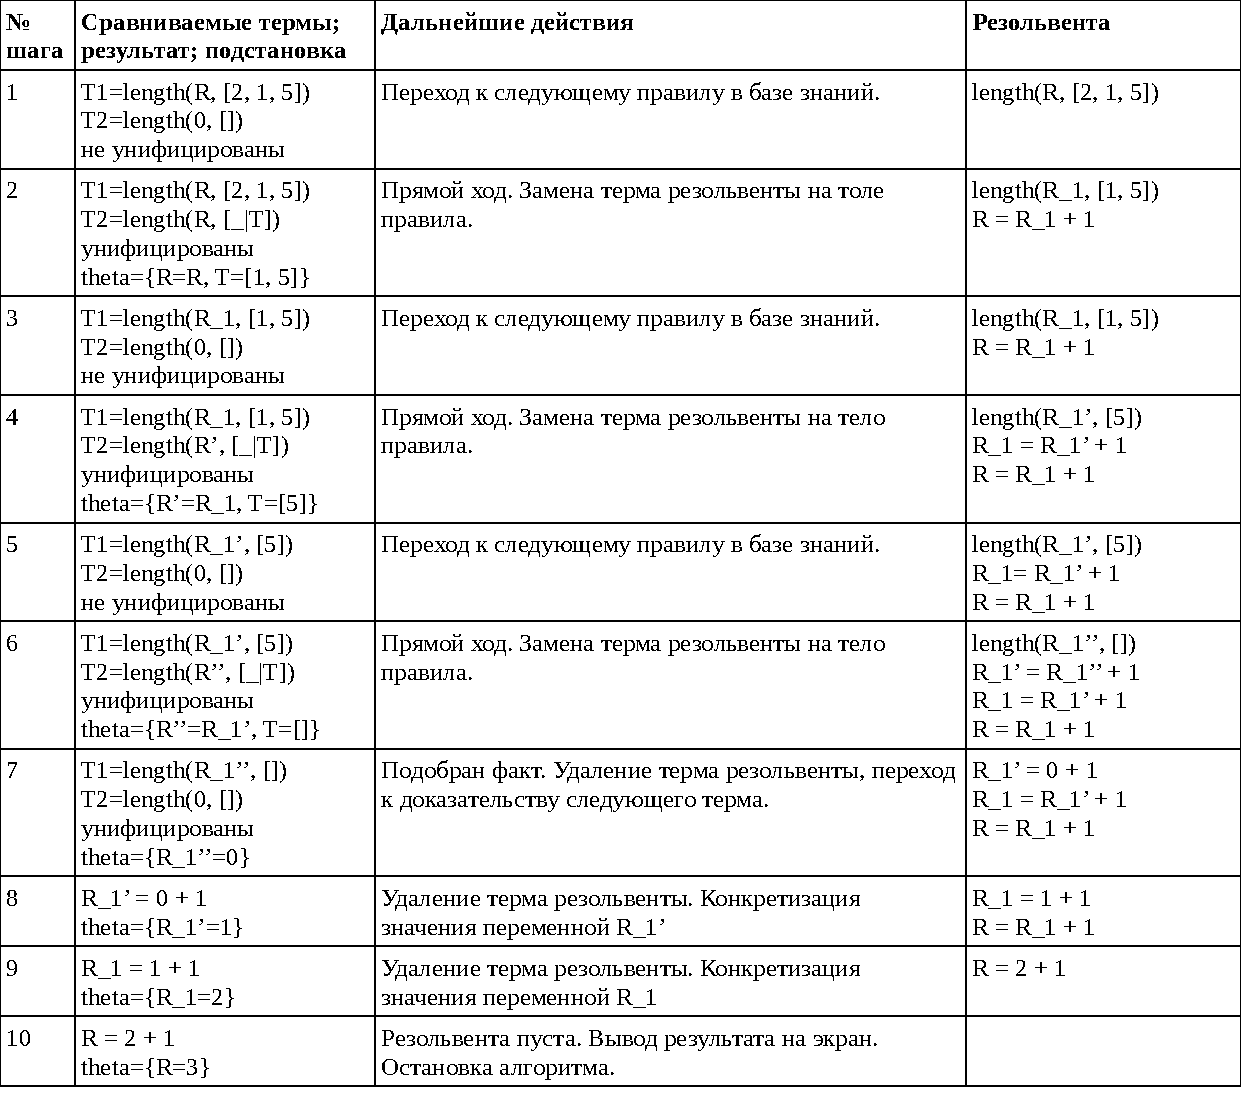
\includegraphics[width=\linewidth]{table1.pdf}
\end{center}

Порядок поиска ответа для 2 варианта:

\begin{center}
	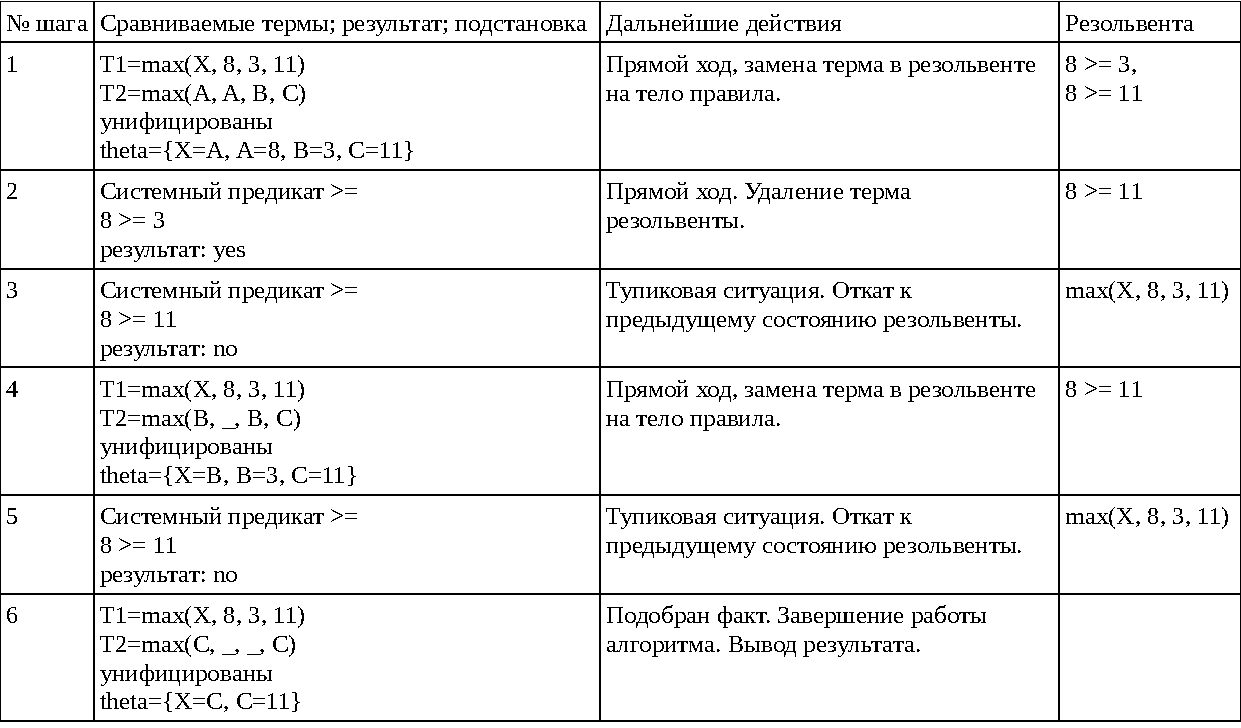
\includegraphics[width=\linewidth]{table2.pdf}
\end{center}


\backmatter % Здесь заканчивается нумерованная часть документа и начинаются ссылки и
{\large\section*{Заключение}}

В ходе работы были приобретены навыки построения предметной области, разработки и оформления программы на Prolog. Были изучены принципы, логика формирования программы и отдельные шаги выполнения программы написанной на языке Prolog. Были освоены принципы и правила сопоставления, отождествления и унификации.

%% % Список литературы при помощи BibTeX
% Юзать так:
%
% pdflatex report
% bibtex report
% pdflatex report

\bibliographystyle{utf8gost780u}
\bibliography{report}

\end{document}